%%%%%%%%%%%%%%%%%%%%%%%%%%%%%%%%%%%%%%%%%
% Short Sectioned Assignment LaTeX Template Version 1.0 (5/5/12)
% This template has been downloaded from: http://www.LaTeXTemplates.com
% Original author:  Frits Wenneker (http://www.howtotex.com)
% License: CC BY-NC-SA 3.0 (http://creativecommons.org/licenses/by-nc-sa/3.0/)
%%%%%%%%%%%%%%%%%%%%%%%%%%%%%%%%%%%%%%%%%

% \documentclass[paper=a4, fontsize=11pt]{scrartcl} % A4 paper and 11pt font size
\documentclass[11pt, a4paper]{book}
\usepackage[T1]{fontenc} % Use 8-bit encoding that has 256 glyphs
\usepackage[utf8]{inputenc}
\usepackage{fourier} % Use the Adobe Utopia font for the document - comment this line to return to the LaTeX default
\usepackage{listings} % para insertar código con formato similar al editor
\usepackage[spanish, es-tabla]{babel} % Selecciona el español para palabras introducidas automáticamente, p.ej. "septiembre" en la fecha y especifica que se use la palabra Tabla en vez de Cuadro
\usepackage{url} % ,href} %para incluir URLs e hipervínculos dentro del texto (aunque hay que instalar href)
\usepackage{graphics,graphicx, float} %para incluir imágenes y colocarlas
\usepackage[gen]{eurosym} %para incluir el símbolo del euro
\usepackage{cite} %para incluir citas del archivo <nombre>.bib
\usepackage{enumerate}
\usepackage{hyperref}
\usepackage{graphicx}
\usepackage{tabularx}
\usepackage{booktabs}

% Matemáticas 
\usepackage{amsmath, amsthm, amssymb} % Paquetes matemáticas
\usepackage{mathtools}                % Añade mejoras a amsmath
\usepackage[mathscr]{eucal} 		  % Proporciona el comando \mathscr para
                                      % fuentes de tipo manuscrito en modo matemático sin sobreescribir el comando \mathcal
% TEOREMAS Y ENTORNOS ASOCIADOS

% \newtheorem{theore<m}{Theorem}[chapter]
\newtheorem*{teorema*}{Teorema}
\newtheorem{teorema}{Teorema}[chapter]
\newtheorem{proposicion}{Proposición}[chapter]
\newtheorem{lema}{Lema}[chapter]
\newtheorem{corolario}{Corolario}[chapter]
\newtheorem{axioma}{Axioma}

\theoremstyle{definition}
\newtheorem{definicion}{Definición}
\newtheorem{ejemplo}{Ejemplo}[chapter]

\usepackage[table,xcdraw]{xcolor}
\hypersetup{
	colorlinks=true,	% false: boxed links; true: colored links
	linkcolor=black,	% color of internal links
	urlcolor=cyan		% color of external links
}
\renewcommand{\familydefault}{\sfdefault}
\usepackage{fancyhdr} % Custom headers and footers
\pagestyle{fancyplain} % Makes all pages in the document conform to the custom headers and footers
\fancyhead[L]{} % Empty left header
\fancyhead[C]{} % Empty center header
\fancyhead[R]{Elena Merelo} % My name
\fancyfoot[L]{} % Empty left footer
\fancyfoot[C]{} % Empty center footer
\fancyfoot[R]{\thepage} % Page numbering for right footer
%\renewcommand{\headrulewidth}{0pt} % Remove header underlines
\renewcommand{\footrulewidth}{0pt} % Remove footer underlines
\setlength{\headheight}{13.6pt} % Customize the height of the header

\usepackage{titlesec, blindtext, color}
\definecolor{gray75}{gray}{0.75}
\newcommand{\hsp}{\hspace{20pt}}
\titleformat{\chapter}[hang]{\Huge\bfseries}{\thechapter\hsp\textcolor{gray75}{|}\hsp}{0pt}{\Huge\bfseries}
\setcounter{secnumdepth}{4}
\usepackage[Lenny]{fncychap}


\begin{document}

	% Plantilla portada UGR
	\begin{titlepage}
\newlength{\centeroffset}
\setlength{\centeroffset}{-0.5\oddsidemargin}
\addtolength{\centeroffset}{0.5\evensidemargin}
\thispagestyle{empty}

\noindent\hspace*{\centeroffset}\begin{minipage}{\textwidth}

\centering

\includegraphics[width=0.9\textwidth]{logos/logo_ugr.jpg}\\[1.4cm]

\textsc{ \Large TRABAJO DE FIN DE GRADO\\[0.2cm]}
\textsc{ DOBLE GRADO EN INGENIERÍA INFORMÁTICA Y MATEMÁTICAS}\\[1cm]

{\Huge\bfseries Análisis de redes causales en deportes de equipo \\}
\noindent\rule[-1ex]{\textwidth}{3pt}\\[3.5ex]
\end{minipage}

\vspace{2.5cm}
\noindent\hspace*{\centeroffset}
\begin{minipage}{\textwidth}
\centering

\textbf{Autora}\\ {Elena Merelo Molina}\\[2.5ex]
\textbf{Directores}\\ {Juan Julián Merelo Guervós, Úrsula Torres Parejo}\\[2cm]
\textsc{Escuela Técnica Superior de Ingenierías Informática y de Telecomunicación}\\
\textsc{Facultad de Ciencias}\\
\textsc{---}\\
Granada, septiembre de 2022
\end{minipage}
\end{titlepage}


	% Plantilla prefacio UGR
	\thispagestyle{empty}

\begin{center}
{\large\bfseries Análisis de redes causales en deportes de equipo }\\
\end{center}
\begin{center}
Elena Merelo Molina\\
\end{center}

%\vspace{0.7cm}

\vspace{0.5cm}
\noindent{\textbf{Palabras clave}: \textit{software libre, redes bayesianas, redes causales, 
entropía, entropía de Tsallis, inferencia estadística, teorema de Bayes}}
\vspace{0.7cm}

\noindent{\textbf{Resumen}\\
	
}
\cleardoublepage

\begin{center}
	{\large\bfseries Same, but in English}\\
\end{center}
\begin{center}
	Elena Merelo Molina\\
\end{center}
\vspace{0.5cm}
\noindent{\textbf{Keywords}: \textit{open source}, \textit{bayesian networks}, \textit{causal networks}, 
\textit{entropy}, \textit{Tsallis entropy}, \textit{inference}, \textit{statistics}, \textit{Bayes theorem}
}
\vspace{0.7cm}

\noindent{\textbf{Abstract}\\

}
\cleardoublepage

\thispagestyle{empty}

\noindent\rule[-1ex]{\textwidth}{2pt}\\[4.5ex]

D. \textbf{Juan Julián Merelo Guervós}, Profesor del departamento de ATC, y D. \textbf{Úrsula Torres Parejo}, 
Profesora del Departamento de Estadística e Investigación Operativa

\vspace{0.5cm}

\textbf{Informo:}

\vspace{0.5cm}

Que el presente trabajo, titulado \textit{\textbf{Análisis de redes causales en deportes de equipo}},
ha sido realizado bajo mi supervisión por \textbf{Elena Merelo Molina}, y autorizo la defensa de dicho 
trabajo ante el tribunal que corresponda.

\vspace{0.5cm}

Y para que conste, expiden y firman el presente informe en Granada a septiembre de 2022.

\vspace{1cm}

\textbf{El/la director(a)/es: }

\vspace{5cm}

\noindent \textbf{(Juan Julián Merelo Guervós, Úrsula Torres Parejo)}

\chapter*{Agradecimientos}

A mis padres, por creer en mí cuando yo no lo hago, animarme a continuar las innumerables veces que tiro la 
toalla y ser tan fundamentales en mi día a día, darle un toque especial y hacerlo mucho mejor todo. Por estar 
siempre ahí, haberme dado y aportado tantísimo en mi vida. A mis hermanas, por apoyarme y aceptarme. A la 
tienda Alehop, porque sin el ventilador que les compramos habría sido mucho más pesado trabajar durante 
esta horrible ola de calor contínua que llamamos verano en Granada. Al Mercadona, por vender chocolate y 
queso tan rico. A las personas que han aparecido aquí y allí, o me han acompañado y ayudado desde el principio 
en esta carrera de fondo; iluminado el camino por este túnel larguísimo que es el doble grado, y que más 
veces de las que no se sentía más cueva o pozo que otra cosa. 




	% Índice de contenidos
	\newpage
	\tableofcontents

	% Índice de imágenes y tablas
	\newpage
	\listoffigures

	% Si hay suficientes se incluirá dicho índice
	\listoftables 
	\newpage

	% Introducción 
	\chapter{Introducción}

En este capítulo se describen la motivación del proyecto y los objetivos que
se quieren alcanzar durante el desarrollo, así como una introducción histórica al
a la aplicación del análisis al fútbol y las redes bayesianas. 

\section{Motivación}
%¿Por qué queréis hacer este TFG? ¿A quién ayuda? ¿Quién lo usaría? 
%¿Qué solución proponéis? La ingeniería del software trata de resolver 
%problemas, no de hacer aplicaciones, y los problemas deben estar antes que nada.

El fútbol es un deporte de equipo  \textit{complicado}. Suponiendo que 
jueguen veintidós personas, como parte del equipo técnico habrá que 
decidir quiénes jugarán, dónde se posicionará cada uno, cuándo y qué 
cambios se harán, si se aboga más por una táctica defensiva u ofensiva, 
así como en qué hacer incidencia en los entrenamientos, entre otros. 
Son bastantes las variables que entran, literalmente, en juego. 

% por parte de quién, qué podría ser usado??? quitar lo del jugador
% poner preguntas que surgen. SER MÁS ESPECÍFICO.
Surgen, pues, de manera natural preguntas en torno a la práctica de 
este deporte alrededor del cual gira todo un mundo, y la importancia 
de las decisiones que se van tomando tanto dentro como fuera del 
campo: Si a un equipo le va mal en un campeonato, se echa al entrenador, pero ¿de quién 
es realmente 'la culpa'?
Principalmente,  el presente trabajo pretende ayudar a un 
entrenador que , durante un partido, quiera saber el efecto de un 
cambio de alineación, técnica o formación, y tras el mismo saber 
qué mejorar, en qué trabajar más, qué ha causado un gol o pérdida 
de la posesión, o a un analista de datos que, antes de un partido, 
estudia al equipo rival o al propio, a nivel individual o colectivo: 
el número de contactos de cada jugador con el balón, el porcentaje 
de acierto tanto tirando a gol como pasando a un compañero, la 
dirección, el número de ataques realizados por sector del campo, 
las conexiones entre jugadores,...

No obstante, podría ser usado también por aficionados, personas que apuestan, analistas tácticos, técnicos o de rendimiento físico, y no necesariamente de un equipo profesional que tenga muchos medios. Pero de esto hablaremos en profundidad en próximos capítulos, cuando establezcamos los objetivos, clientes e historias de usuario.
% no me convence el final, me falta responder bien las últimas preguntas

\section{Objetivos del trabajo} \label{sect:goals}

Dado el problema anterior, los objetivos a resolver son:

\begin{enumerate}
    \item \label{obj:1} Crear una herramienta para que personas del equipo técnico de un equipo de fútbol, como analistas de datos, analistas técnicos, analistas de rendimiento 
    físico o entrenadores, puedan tomar decisiones en base al estudio que se haga antes, durante 
    o después de un partido. 
    \item \label{obj:2} Entender cómo se pueden aplicar redes causales e inferencia 
    bayesiana en deportes de equipo, y adaptar resultados en ese campo a 
    los tipos de datos que existen aquí.
\end{enumerate}



Este proyecto es software libre, y está liberado con la licencia \cite{gplv3}.


	% Descripción del problema y hasta donde se llega
	\chapter{Descripción del problema}

Este proyecto tiene como idea ayudar desde los jugadores hasta 
el cuerpo técnico del equipo: entrenadores, director técnico, preparadores 
físicos y analistas tácticos,también conocidos como 'scouting'.

\section{Perfiles dentro del análisis de fútbol}

scout, analista, ojeador 


\section{Métricas en el fútbol moderno: concepto, análisis y uso}

\subsection{Expected goals o Goles esperados, xG}


\subsection{Expected assists o Asistencias esperadas, xA}


\subsection{Expected points o Puntos esperados,xP o xPts}


\subsection{Pases Permitidos por Acción Defensiva,PPDA}


\section{Metodología}


\section{Clientes}
A su vez, dentro del análisis de fútbol, podemos destacar los siguientes roles:

\begin{itemize}
    \item Analista táctico: se encarga de estudiar los equipos y cómo 
    se desenvuelven en los diferentes partidos. Querrá obtener un análisis 
    del propio equipo y de los rivales.
    \item Scouter: es la persona encargada de la búsqueda y captación 
    de jugadores. Querrá encontrar los jugadores que necesita el equipo 
    o el club, por lo que analiza sus cualidades y posibilidades de 
    integración al equipo, desde su rendimiento futbolístico hasta el 
    económico.
    \item Analista de datos: toma la información estadística de 
    cada partido tanto en lo individual como en lo colectivo. 
    Establece relaciones para encontrar respuestas o ideas que 
    puedan colaborar con la toma de decisiones del club referentes 
    a lo táctico, lo técnico y lo económico, para el modelo de 
    juego del equipo o para la compra y venta de jugadores. Por ejemplo: del 
    equipo femenino de Noruega. 
    \item Persona que apuesta: querrá inferir el resultado de un partido, 
    quién marcará y así, una vez se publiquen los jugadores. 
    \item Entrenador: querrá saber a quién sacar durante un partido, los 
    cambios, dónde poner a quién. Por ejemplo: entrenadora principal y 
    segunda entrenadora del Club de Fútbol Internacional del Granada.
    \item Matemático ?
    \item Informático ?
    \item Aficionado  ?
\end{itemize}

Manteniendo esto en mente, nuestra solución 
podría ser usada por ellos. Vemos entonces 
que el trabajo se puede enfocar de diversas 
maneras, y conforme avancemos habremos de descartar algunas y 
quedarnos con otras, quedando todo debidamente justificado. Dependerá de los 
datos que se encuentren disponibles, y la necesidad que haya en el mercado. 
Normalmente y si consultamos la literatura, los análisis son estáticos; 
rendimiento y mapas de calor de un jugador, desde dónde se ha lanzado más 
a portería, etc. pero no hay tanto estudiado en cuanto a causalidad.

\section{Historias de usuario}  




	% Estado del arte
	% 	1. Crítica al estado del arte
	% 	2. Propuesta
	\chapter{Estado del arte}
La historia del análisis de fútbol comienza en 1950, cuando Charles Reep \cite{reep-bio}, teniente coronel de 
la \textit{Royal Air Force} británica y contable, empezó a 
registrar sistemáticamente los eventos que tenían lugar a lo largo de un partido de Swindon Town. Con ello, no pretendía 
únicamente tener detalle de lo que había ocurrido, sino también saber por qué pasaba y qué podían aprender los 
equipos de los datos, para mejorar su juego. Tras décadas, llegó a la conclusión de que el mayor número 
de goles resultaba de posesiones de tres pases o menos, por lo que aludía que los equipos debían simplificar 
sus tácticas para llegar a portería más rápido.

El problema de Reep no fue su recolección de datos, sino su análisis; podría haberse preguntado sobre 
la tasa de goles en posesiones de varias distancias, o cómo se desarrollaron exactamente esas 
posesiones de tres pases. 

Otro pionero en el uso de datos en el deporte fue \href{http://www.riazhaq.com/2022/08/remembering-salam-qureishi-pillar-of.html}{Abdus Salam Qureishi}, 
filántropo e informático en Sillicon Valley, hacía \textit{datascouting} en la reconstrucción de los 
\href{https://www.dallascowboys.com/}{Dallas Cowboys}, un equipo profesional de fútbol americano de los años 60 \cite{chazan2020sports}.

En los años 70, \href{https://es.wikipedia.org/wiki/Valeri_Lobanovski}{Valeri Lobanovski} fue un jugador y entrenador de 
fútbol ucraniano que formalizó el cuerpo técnico moderno y la captura de eventos en el fútbol del equipo \href{https://es.wikipedia.org/wiki/F._C._Dinamo_de_Kiev}{Dinamo de 
Kiev}. Declaraba que ``Hoy en día los jugadores no pueden quejarse, saben que mañana después del partido habrá colgada una hoja con 
las cifras que describen en detalle su juego" \cite{kilpatrick2011inverting}.

En 1996, \href{https://es.wikipedia.org/wiki/Opta_Sports}{Opta} empezó a acumular datos de partidos para la 
\textit{Premier League} inglesa. Ello incluía todas las estadísticas a las que un aficionado al fútbol está 
acostumbrado: número de pases, número de regateos, distancia recorrida, por ejemplo. Este podría considerarse 
el punto de comienzo del análisis de fútbol moderno. Desde 2019, se llama \href{https://www.statsperform.com/}{Stats Perform}, y 
es todo un referente a la hora de análisis de datos de deportes, incorporando inteligencia artificial.

En 2003, Michael Lewis lanzó el libro \href{https://en.wikipedia.org/wiki/Moneyball}{Moneyball}, el cual tuvo una gran 
influencia también fuera de Estados Unidos. Trata sobre cómo
un equipo de béisbol de bajo presupuesto se convirtió en uno de los mejores, usando estadísticas para reclutar a jugadores 
con habilidades hasta entonces minusvaloradas, como el \href{https://en.wikipedia.org/wiki/On-base_percentage}{porcentaje de veces que un bateador llega a una base}, o 
la \href{https://en.wikipedia.org/wiki/Slugging_percentage}{productividad de bateo} \cite{moneyball-ev}. El lanzamiento del 
libro fomentó que se generaran \href{https://thesportjournal.org/article/an-examination-of-the-moneyball-theory-a-baseball-statistical-analysis/}{preguntas} en torno al empleo de datos en deportes de equipo. 

A su vez, en 2005 hubo muchos intentos de relacionar redes complejas y fútbol \cite{lee2005passes}, 
e incluso en el 2004 se lanzó un desafío en la lista redes \cite{Bundio_Matías_2008} para predecir el resultado de la Eurocopa usando 
redes sociales. En cualquier caso, tanto el estallido del análisis de redes sociales como el libro contribuyeron 
a la expansión de este campo.

En los últimos años ha habido una revolución en el análisis de la organización 
y rendimiento de los equipos de fútbol y sus jugadores, por lo que es posible tener acceso a todos los 
eventos que ocurren en el campo, tales como pases, disparos o goles, todo ello con las coordenadas 
exactas de tiempo y posición, y el jugador responsable de cada evento. Por otro lado, también es 
posible llevar un registro de las posiciones de todos los jugadores en el campo, junto con el balón, 
lo que permite determinar la posición, velocidad y aceleración de cada jugador, y dando información 
muy útil sobre su desempeño físico y táctico. 

No obstante, los avances más determinantes e importantes tienen que ver con la posibilidad de aplicar o 
definir nuevos métodos y herramientas. En ese sentido, se pueden entender los roles de los jugadores 
como un todo, no solo como componentes aisladas sin interacciones entre ellos. Consecuentemente, es 
posible contruir redes de pases compuestas por nodos, correspondientes a los jugadores, y enlaces, 
que representan los pases entre ellos. Esta organización está además lejos de ser 
aleatoria. El análisis de la evolución de las redes de pases ha mostrado que sus propiedades 
cambian continuamente a lo largo de un partido y que eventos importantes tales como goles 
pueden afectar la organización de la red \cite{spatial-and-temporal-entropies}.

Asimismo, durante la última década las redes bayesianas \ref{def:BN} se han popularizado en el campo 
de la inteligencia artificial, y hay numerosos estudios que buscan predecir los resultados 
de partidos de fútbol empleándolas, para lo que construyen diferentes modelos \cite{prediction-barcelona}.
En \cite{razali-2017} consiguen una precisión predictiva del 75.09\%. \cite{dolores} introduce el uso 
de calificaciones dinámicas \ref{subsect:ratings} y redes bayesianas híbridas \ref{def:hybrid_BN} para hacer una predicción del resultado de un 
partido entre dos equipos \textit{a} y \textit{b} a partir de datos históricos de partidos 
en los que no participan ni \textit{a} ni \textit{b}. Ello nos muestra 
el increíble potencial que tienen estas redes también, y no solo las más tradicionales 
redes complejas \ref{def:CN} \cite{caldarelli2007scale}. 

A diferencia de los sistemas simples, muy pocas metodologías tratan la evaluación de la confiabilidad de
sistemas complejos, especialmente los configurados como redes, donde es difícil tomar en
consideración los diferentes vínculos y factores que pueden afectar la disponibilidad y confiabilidad de tales
sistemas En este contexto, las redes bayesianas permiten el
modelado de sistemas configurados como red y el cálculo de probabilidades marginales de la
nodos del sistema utilizando probabilidades previas y condicionales \cite{bn-and-cn}.

Adicionalmente, hay estudios \cite{smart-data} que ponen un gran énfasis 
en aplicar conocimiento causal al proceso de desarrollo del modelo, basándose 
en los datos que son necesarios para la predicción. De esa manera, consiguen predicciones precisas 
del cambiante rendimiento de equipos de fútbol. El modelo permite predecir, antes de que empiece 
una temporada, los puntos totales en la liga que se espera un equipo acumule a lo largo de la temporada, lo 
que supone un cambio de perspectiva con respecto a los artículos mencionados con anterioridad, y en su 
metodología construye y trabaja sobre la literatura anterior, extendiéndola.

Por otro lado, hay vertientes que hacen análisis de fútbol desde la inferencia estadística, desde 
el \textit{machine learning}, o ambos \cite{ML-inference}. En este \textit{paper}, muestran que 
los equipos están caracterizados por dónde en el campo realizan pases, y se 
pueden identificar por la manera en que pasan el balón. Usando mapas de calor de las localizaciones 
de los pases, consiguen una precisión del 87\% en una clasificación de veinte equipos. Emplean 
además la localización de los pases a lo largo de una posesión del balón para predecir tiros a 
puerta. Finalmente, usan los pesos del modelo de predicción para categorizar a los jugadores 
según el valor de sus pases. Nos muestra una vez más la diversidad que existe en el estudio 
y análisis del fútbol; no hay límites en cuanto a lo que se puede considerar y obtener.

\cite{entropy-analysis} afirma que para optimizar su rendimiento, un 
equipo debe mantener un equilibrio entre orden u organización, el cual 
propicia la cooperación entre sus miembros, y desorden o desorganización, que confunde 
al oponente y favorece el mantener un cierto grado de libertad. Para medir, usan entropía de 
Tsallis \ref{def:tsallis_entropy} a partir de los pases entre los jugadores, y concluyen que la posición de un equipo 
al final de la temporada está correlada con la entropía del mismo. 

Más específicamente, saber quién pasa el balón a quién significa reducir la entropía \ref{def:entropy} de los pases y maximizar 
la comunicación y cooperación entre los jugadores del equipo. A su vez, esto implicaría limitar sus 
grados de libertad al mover la pelota y sorprender al oponente, lo que expondría al equipo a contraataques. El precio 
pues de maximizar la certeza de los pases puede ser un comportamiento predecible y hacer al equipo vulnerable. Lo más importante 
de este \textit{paper} es que reivindica que el rendimiento de un equipo de fútbol puede 
ser modelado usando la entropía de sus pases de balón.

Y no solo eso, \cite{spatial-and-temporal-entropies} cuantifica la entropía espacial y temporal de 
equipos de fútbol y sus jugadores, también mediante interacciones basadas en pases. Sus resultados 
muestran que la entropía espacial cambia de acuerdo con la posición de los jugadores en el campo, y la 
organización de las redes de pases cambian a lo largo de un partido. 

\cite{network-analysis} fue uno de los primeros en investigar la entropía entre los jugadores de un equipo de 
fútbol. Analizan el desempeño y estilo de juego de la selección española en los mundiales del 2010 desde una 
perspectiva temporal, con lo que medidas globales como el número de pases consecutivos o el número de 
pases por minuto reflejan el éxito de un equipo en imponer su forma de juego.
Así, España consigue tener mayor posesión del balón y pases completados, lo que es una buena estrategia defensiva 
al privar al otro equipo de influenciar en el juego. Esto en último lugar determina el resultado final del partido, 
si bien es discutible la necesidad de tener tanto tiempo el balón, sin muchas veces avanzar a puerta. En el 
último partido muestran que la precisión disminuye y el juego es menos elaborado, al introducirse 
más emoción y nervios.

Pero, ¿cómo medimos la calidad de un equipo? No hay muchos artículos aplicando redes causales a partidos de 
fútbol. \cite{cerqueira} muestra que las estrategias ofensivas son más influyentes que las defensivas.



 
	
	\chapter{Planificación}
En este capítulo describiremos cómo nos hemos organizado y repartido el trabajo.

\section{Temporización}

\section{Seguimiento del desarrollo}


	% Análisis del problema
	% 1. Análisis de requisitos
	% 2. Análisis de las soluciones
	% 3. Solucion propuesta
	% 4. Análisis de seguridad
	\chapter{Desarrollo teórico}
En este capítulo estableceremos la base matemática del proyecto. Principalmente nos basaremos en 
los libros \textit{Advanced Data Analysis
from an Elementary Point of View} \cite{ada} y \textit{Probabilistic Networks for Practitioners — A
Guide to Construction and Analysis of Bayesian
Networks and Influence Diagrams} \cite{pgm}, junto con el capítulo \textit{An overview of the representation and 
discovery of causal relationships using bayesian networks} \cite{cooper}.

\subsection{Fundamentos de grafos}
Un grafo es un par $G = (V, E)$, donde $V$ es un conjunto finito de vértices distinguibles y 
$E \subseteq V \times V$ es un conjunto de aristas. Un par ordenado $(u, v) \in E$ denota un borde dirigido
del vértice $u$ al vértice $v$, y se dice que $u$ es padre de $v$ y $v$ hijo de $u$. Los bordes dirigidos 
se representarán como flechas, y los bordes no dirigidos como líneas. 

\begin{figure}[h!]
    \centering
     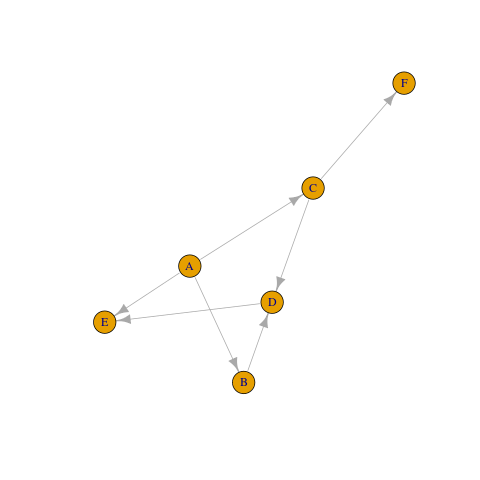
\includegraphics[width=\textwidth]{./img/dag.png}
     \caption{Ejemplo de grafo dirigido acíclico (DAG)}
     \label{img:dag1}
    \end{figure}

Una forma relativamente natural de ver un partido de fútbol es como una secuencia de 
pases entre jugadores e intercepciones, que terminan en una resolución. 

Si $E$ no contiene bordes no dirigidos, entonces $G$ es un grafo dirigido, y si $E$ no 
contiene bordes dirigidos, entonces es un grafo no dirigido. Un camino $ \langle v_{1},...,v_{n} \rangle $ 
es una secuencia de vértices distinguidos tales que $u \rightarrow v$, $v \rightarrow u$ o $u - v$ para 
cada $i= 1,..., n-1$. La longitud del camino es $n-1$. El camino es dirigido si $v_{i} \rightarrow v_{i+1}$ 
para cada $i= 1,..., n-1$; $v_{i}$ es por tanto un ancestro de $v_{j}$ y $v_{j}$ es un descendiente de 
$v_{i}$ para cada $j > i$. 

Un grafo $G= (V, E)$ está conectado si para cada par ${u, v} \subseteq V$ hay un camino 
$\langle u,...,v \rangle$ en $G$. Un ciclo es un camino, 
$\langle u,...,v \rangle$ de longitud mayor que dos (excepto el caso $v_{1} = v_{n}$); un grafo 
dirigido sin ciclos dirigidos es el ya mencionado DAG. 

\subsection{Modelos gráficos}
A un nivel estructural o cualitativo, los modelos de redes probabilísticas son grafos cuyos vértices 
representan variables y funciones, y los bordes representan distintos tipos de relaciones entre ellas. 

\subsubsection{Variables}
Una variable representa un conjunto exhaustivo de eventos mutuamente excluyentes, conocidos como dominio 
de la variable. Estos eventos también se pueden llamar estados, niveles, valores, elecciones o opciones. 
El dominio de una variable puede ser discreto o contínuo; los dominios discretos son siempre finitos. 
Usaremos letras mayúsculas para denotar variables o conjuntos de variables, y letras minúsculas para sus 
valores. Consecuentemente, $X = x$ puede denotar el hecho de que la variable $X$ toma el valor $x$ o que 
el conjunto de variables $X = (X_{1},...,X_{n})$ toma el vector de valores $x = (x_{1},...,x_{n})$. 
Con $dom(X)= (x_{1},...,x_{||X||})$ denotaremos el dominio de $X$, donde $||X|| = |dom(X)|$ es el número 
de posibles valores de $X$. Si $X = (X_{1},...,X_{n})$, entonces $dom(X)$ es el producto cartesiano sobre 
los dominios de las variables en $X$, $$dom(X)=dom(X_{1})\times ... \times dom(X_{n})$$, y por lo tanto 
$||X|| = \prod_i ||X_{i}||$. Para dos (conjuntos de) variables $X$ e $Y$ escribiremos $dom(X \cup Y)$ 
o $dom(X,Y)$ para denotar $dom(X) \times dom(Y)$.

Usaremos la noción de variable y vértice o nodo de manera indistinta.  

\subsection{Causalidad}
La causalidad tiene un papel muy importante en el proceso de construcción de modelos de redes 
probabilísticas. Una variable $X$ se dice que es una causa directa de $Y$ si al establecer el valor 
de $X$ por la fuerza, el valor de $Y$ cambia y no hay otra variable $Z$ que sea causa directa de 
$Y$ tal que $X$ es causa directa de $Z$. Para representar correctamente las relaciones de dependencia 
e independencia que existen en un conjunto de variables 
del dominio de un problema, es muy útil tener las relaciones de causalidad que hay entre las variables 
representadas como enlaces dirigidos desde las causas 
a los efectos. Esto es, si $X$ es una causa directa de $Y$, tenemos que asegurarnos de añadir un enlace 
desde $X$ a $Y$. 

En las siguientes subsecciones discutiremos cada uno de las posibles formas de conexión que pueden aparecer en una red.

\section{Probabilidades} 
% issue #61
\section{Fundamentos de redes probabilísticas}
%¿Por qué nos interesa esto? ¿Qué vamos a hacer con ellas?
%¿Qué tienen que ver con los grafos? O igual simplemente haz una referencia.
Las redes probabilísticas son modelos gráficos de interacciones (causales) entre una
conjunto de variables, donde las variables se representan como vértices o nodos de un 
gráfico y las interacciones (dependencias directas) como aristas dirigidas (también
enlaces y arcos) entre los vértices. Cualquier par de vértices no conectados indican 
independencia (condicional) entre las variables representadas
por estos vértices en circunstancias particulares que se pueden leer fácilmente desde el
grafo. 

Los grafos han demostrado ser un lenguaje muy intuitivo para representar
tales declaraciones de dependencia e independencia, y por lo tanto proporcionan un excelente
lenguaje para comunicar y discutir las relaciones entre las 
variables del dominio del problema, las cuales se pueden representar de forma muy compacta 
mediante grafos dirigidos acíclicos (DAG).

No obstante, la propiedad que distingue a la inferencia en redes probabilísticas
de otros paradigmas de razonamiento automático es su capacidad para hacer razonamientos intercausales: 
obtener evidencia que apoye una sola hipótesis o un subconjunto de
hipótesis conduce a la disminución de la creencia en las otras con las que compiten y para las que no se 
han encontrado unas bases que las soporten. Por ejemplo, hay un gran número de posibles causas por las 
que un coche puede no arrancar, entre ellas falta de combustible. Observar que el indicador de combustible 
indica que no hay combustible proporciona una fuerte evidencia de que la falta de combustible es la causa 
del problema, a la vez que la creencia en otras causas posibles disminuye sustancialmente. La capacidad 
de las redes probabilísticas para realizar automáticamente tal inferencia intercausal de manera adecuada 
es una contribución clave a su poder de razonamiento.

La parte gráfica de una red probabilística se conoce como aspecto cualitativo, mientras que la 
parte probabilística o numérica constituye su aspecto cuantitativo. Nos dedicaremos primeramente al aspecto 
cualitativo de las redes probabilísticas.

\section{Redes causales}

\section{Fundamentos de redes bayesianas}
Las redes bayesianas nos ayudan a modelar y entender las muchas variables que informan nuestro proceso de 
toma de decisiones. Las decisiones más complejas están normalmente basadas en una multitud de factores o 
variables. Por ejemplo, para el presidente de un equipo de fútbol \ref{hu:presidente}, podemos 
mapear la decisión que tiene que tomar y las diferentes variables usando 
una red bayesiana, esto es, un modelo gráfico que captura la relación entre variables que están bajo 
supuestos de causalidad o influencia \cite{things-to-know-BN}.

Básicamente entonces, \textbf{una red bayesiana es un diagrama que 
usa flechas o arcos dirigidos para mostrar cómo distintos factores, representados por nodos elípticos, se 
influencian los unos a los otros.} Cada nodo viene con una tabla de probabilidades condicionadas, la cual refleja las 
posibilidades de varios desenlaces, provenientes de las influencias que le afectan directamente. Una vez 
la estructura del grafo y dicha tabla han sido definidas, hay algoritmos estándar que 
calculan los estados de las variables desconocidas basándose en los estados de las variables conocidas en el
modelo \cite{learning-algorithms-BN-comparison}, \cite{BN-achilles-heel}, \cite{different-algorithmic-schemes}.

Una de las razones por las que las redes bayesianas son tan potentes es que pueden realizar inferencias 
tanto predictivas como diagnósticas. Por ejemplo, podemos por un lado predecir la posición en la liga de un equipo para 
un valor dado (observación) de rendimiento, y por otro ingresar un estado de posición en la 
liga como observación para examinar qué nivel de desempeño del equipo podría explicarla. Estos algoritmos estándar son
llamados algoritmos de "propagación bayesiana" \cite{Cano2004}, \cite{more-algorithms}, \cite{back-prop} porque se basan en el teorema de Bayes, en el que la 
probabilidad de una variable desconocida se actualiza después de que se obtenga evidencia relevante para esa variable \cite{prop-alg}.

Las clases de causalidad que producen redes bayesianas son:
\begin{itemize}
    \item \textbf{Cadena causal}: describe variables que tienen un efecto dominó las unas sobre las otras. Por ejemplo, \textit{cambios en la calidad de 
    los jugadores} tiene impacto sobre el \textit{desempeño del equipo} que a su vez influencia la \textit{posición en la liga}. 
    Esto quiere decir que la \textit{posición en la liga} es independiente de los \textit{cambios en la calidad de los jugadores} una vez conocemos el \textit{desempeño del equipo}.\\
    cambios en la calidad de los jugadores $\rightarrow$ Desempeño del equipo $\rightarrow$ Posición en la liga
    \item \textbf{Efecto común}: ocurre cuando dos variables diferentes, tales como \textit{fichajes} y \textit{jugadores vendidos}, tienen influencia sobre una tercera variable tal como 
    \textit{gasto neto en transferencias}. Esto significa que \textit{jugadores vendidos} depende de \textit{fichajes} una vez que conocemos el \textit{gasto neto en transferencias}.\\
    Fichajes $\rightarrow$ Gasto neto en transferencias $\leftarrow$ Jugadores vendidos    
    \item \textbf{Causa común}: tiene lugar cuando dos variables distintas, tales como \textit{posición en la liga} y \textit{asistencia}, se ven influenciados por la misma variable, tal 
    como \textit{desempeño del equipo}. Ello significa que \textit{asistencia} es independiente de \textit{posición en la liga} una vez conocemos \textit{desempeño del equipo}.\\
    Posición en la liga $\leftarrow$ Desempeño del equipo $\rightarrow$ Asistencia
\end{itemize}


\subsection{Construcción de redes bayesianas}
Construir una red bayesiana implica determinar su estructura y su tabla de probabilidades condicionadas. Podemos hacer esto 

\section{Resolución de redes probabilísticas}



	% Desarrollo bajo sprints: 
	% 	1. Permitir registros y login de usuarios
	% 	2. Desarrollo del sistema de incidencias
	% 	3. Desarrollo del sistema de denuncias administrativas y accidentes
	% 	4. Desarrollo del sistema de croquis
	%   5. Instalación de la aplicación de manera automática
	\chapter{Implementación y resultados}
En este capítulo presentaremos los resultados experimentales, y qué nos llevó a ellos, siguiendo 
la metodología ya descrita en \ref{ch:metod}.

\section{Resultados}
Como caso de estudio, nos centraremos en el equipo femenino de Noruega, dejando para trabajos futuros el resto 
de análisis y preguntas que nos podemos plantear.

Más específicamente, usaremos como fuente la 
\href{https://es.uefa.com/womenseuro/news/0258-0e223de64a73-41a64bf308f9-1000--todos-los-resultados/?iv=true}{EURO 
Femenina de la UEFA 2022}, en la cual Inglaterra resultó ganadora, y Noruega perdió 
\href{https://es.uefa.com/womenseuro/match/2032209--england-vs-norway/}{un partido} contra ellas por ocho 
goles a cero (es de notar que seis fueron tan solo en la primera parte), constituyendo uno de los márgenes más 
grandes de victoria (en las fases finales) de la historia 
del campeonato, además de uno de los partidos (nuevamente, de los finales) en los que más goles se han marcado. 
Nuestro objetivo será estudiar por qué ocurrió esto, si podemos verlo reflejado de alguna manera 
en las redes de pases o entropía de ambos equipos. Añadir que luego tampoco pasaron a cuartos de final, al perder 
contra Austria por \href{https://es.uefa.com/womenseuro/match/2032211--austria-vs-norway/}{un gol}. Será interesante 
comparar más a fondo el desempeño de Noruega a lo largo de este campeonato, del cual (para nuestra agradable sorpresa) se 
\href{https://statsbomb.com/articles/soccer/statsbomb-release-free-360-data-womens-euro-2022-available-now/}{
liberaron los datos} el cuatro de agosto, por \href{https://statsbomb.com/}{StatsBomb}, una empresa de 
análisis de fútbol y visualización de datos con sede en el Reino Unido.

Esa derrota fue sorprendente teniendo en cuenta que, si consultamos 
\href{https://www.uefa.com/womenseuro/news/023d-0e16a7c86b1c-05ff0a6fb380-1000--uefa-women-s-euro-facts-and-figures-player-records-most-goals-b/}{
el ``cuadro de honor de la EURO femenina''}, vemos que previamente Noruega ha ganado dos veces esta 
competición, contra una vez que ya ganó Inglaterra; han estado seis veces en la final versus tres que ha 
estado Inglaterra, y nueve veces en semifinales, contra seis de Inglaterra. 
Si consultamos las \href{https://www.uefa.com/womenseuro/statistics/}{estadísticas por equipo y jugadoras}, sin 
duda Inglaterra y Alemania son las que se imponen, apareciendo Noruega únicamente en un quinto puesto en cuanto 
a posesión del balón (52.7 \%, contra un máximo de 63.8\% por parte de España), un sexto puesto por una 
precisión de pases del 79.7\% (contra máximo de un 86.8\%, también de España), y otro quinto puesto por catorce paradas 
de la portera, en comparación con el primer puesto por veintitrés salvadas de Holanda. 

Nuestra pregunta es pues ¿qué les pasó a las noruegas este año? El entrenador (ahora ex-entrenador) Martin Sjögren 
\href{https://www.nrk.no/sport/massiv-kritikk-mot-sjogren-etter-tidenes-storste-norge-tap-1.16034807}{fue muy 
criticado} por no hacer cambios de formación o jugadores en esos primeros 47 minutos en los que volaron goles, 
y al ser ese partido de la EURO 2022 contra Inglaterra la mayor derrota de Noruega en la historia; anteriormente 
habían perdido 0-4 contra Alemania en la Eurocopa de 2009, 0-5 contra China en el mundial de 1999, o 
\href{https://www.nrk.no/sport/norges-landslag-knust-av-nederland--1.15538927}{un 0-7} contra Holanda el año pasado.
\href{https://www.nrk.no/sport/norge-mareritt-mot-england-i-em_-_-dette-er-direkte-pinlig-1.16034607}{Se culpa} a la 
falta de estructura defensiva y presión ofensiva; alegan que empezaron bien, mas una vez Inglaterra marcó el primer gol en 
el minuto 12 no pudieron pararles, y fueron cuesta abajo. Veremos si esto se refleja en los datos obtenidos y por qué 
salió tan mal, considerando en último lugar que Noruega tiene 
\href{https://www.nrk.no/sport/engelsk-forbauselse_-_-jeg-kan-ikke-helt-tro-det-jeg-nettopp-har-vaert-vitne-til-1.16034919}{
jugadoras de los mejores equipos del mundo}. 

No obstante, desde que en Inglaterra tienen a la entrenadora Sarina Wiegman, no 
han perdido los últimos dieciséis partidos. ¿Tan grande es la influencia del entrenador? 
\href{https://www.nrk.no/sport/hvis-det-er-en-plan_-er-den-usynlig-1.16038718}{En este artículo} ponen en evidencia los problemas 
que se han ido arrastrando desde que Sjögren es entrenador, con un rendimiento lejos del esperado (teniendo en 
cuenta la buena prestación de las jugadoras cuando juegan en los equipos en que están fichadas) en las últimas 
competiciones. Conceptualizar y medir cuánto y en qué se diferencia un todo de la suma de sus partes es un desafío no 
trivial. Una posible dirección para abordar esto consiste en cuantificar hasta qué punto la entropía 
del todo no es aditiva  \cite{whole-different}. Se discute que como equipo cometieron errores a la hora de posicionarse, dejaron libre la zona de 
defensa y jugadoras que podrían haber sido decisivas se quedaron aisladas, con lo que abrieron las puertas a 
las inglesas a dominar el juego. 

\href{https://www.nrk.no/sport/norsk-fiasko-i-em_-_-en-varslet-katastrofe-1.16039578}{En el partido contra Austria},
que debían ganar, no hubo un solo disparo a puerta antes del minuto 88, por lo que siguieron siendo una sombra de sí 
mismas, pese a que, en sus palabras, usaron los días posteriores para reconstruir su orgullo y autoestima, y recomponerse 
de tal golpe bajo. No consiguieron estar a la altura, dejar de ser una sombra de ellas mismas, y hubieron de pasar 
63 minutos antes de que el entrenador hiciera un cambio (el gol de Austria fue en el minuto 37). Se cometieron también 
errores aquí y allí, pero está lejos de ser el partido contra Inglaterra. ¿Podremos ver esta diferencia reflejada 
en las redes de pases o entropía del equipo? Principalmente, ¿es problema de la formación 
(en \href{https://www.nrk.no/sport/reiten-ut-mot-sjogren-grep_-_-pa-tide-med-noko-nytt-1.16085631}{la nueva 
entrenadora Hege Riise} afirma que habría sido mejor jugar 4-3-3, en vez de 4-2-3-1), del entrenador, de las 
jugadoras que no supieron coordinarse, o simplemente no están a la altura de Inglaterra? Con este trabajo intentaremos 
encontrar respuestas. 

\section{Elección de fuentes de datos}
Escogemos las de \href{https://github.com/statsbomb/open-data}{StatsBomb}, al contener datos de los partidos y equipos que nos interesaban. Otras opciones disponibles en 
el mercado son \href{https://www.statsperform.com/}{StatsPerform}, para el cual hay que pagar, 
\href{https://fbref.com/en/}{FbRef}, el cual dispone de datos libres, pero para descargarlos y tratar con ellos 
es más aparatoso y manual, aparte de que no tiene los datos temporales ni de los pases con tanto detalle y 
extensión como Statsbomb.

\section{Paquetes de R}
En este apartado describiremos los paquetes de R de los que hemos hecho uso, justificando nuestra elección.

\subsection{Igraph}
La librería y paquete \href{https://igraph.org/r/}{igraph} de R lo hemos escogido por su facilidad a la hora de 
calcular la entropía;está destinada al análisis de redes y consta por tanto de \href{https://kateto.net/netscix2016.html}{funciones sencillas} para calcular 
medidas como \textit{closeness, network density, centrality, betweenness, centralization, robustness, 
efficiency, effectiveness and diversity} sobre grafos, mediante la 
creación de \href{https://igraph.org/r/doc/graph_from_data_frame.html}{``graph dataframes''}, que viene genial 
dado que podemos usarlos con \href{https://www.rdocumentation.org/packages/graphics/versions/3.6.2/topics/plot}{plot} 
y te traza la red, y si aparte quieres usarlos como dataframes para hacer otros cálculos, también se puede. Un ejemplo 
de uso podemos verlo \href{https://github.com/JJ/venice-patrician-social-network/blob/main/patrician-social-network.R}{aquí}, 
programa en el cual nos inspiramos para trazar nuestra red de pases.

\subsection{Devtools}
Si bien la mayoría de los paquetes de R están en \href{https://cran.r-project.org/}{CRAN}, hay muchos que vamos 
a necesitar que se encuentran en Github. \href{https://www.r-project.org/nosvn/pandoc/devtools.html}{devtools} da 
la posibilidad de descargarlos directamente.

\subsubsection{Statsbomb}
\href{https://github.com/statsbomb/StatsBombR}{Este paquete} lo empleamos, una vez decidido que íbamos a hacer 
uso de sus datos, para poder quedarnos con las columnas que nos interesaban y demás operaciones, esto es, \textit{parsear} 
la información. 

\subsection{Tidyverse}
\href{http://www.storybench.org/getting-started-with-tidyverse-in-r/}{Tidyverse} contiene paquetes como 
\href{https://dplyr.tidyverse.org/}{dplyr} que son útiles para manipular, explorar y visualizar datos, y 
prácticamente es un estándar en estadística y ciencia de datos. \href{https://rviews.rstudio.com/2017/06/08/what-is-the-tidyverse/}{Sus ventajas} 
incluyen funciones consistentes y uso a lo largo de todo el \textit{workflow}, lo que se ve reflejado en una 
mayor productividad, y no nos hizo dudar al escogerlo. \href{https://www.r-bloggers.com/2018/09/why-learn-the-tidyverse/}{Más ventajas} incluye 
que carga una \textit{suite} complete y extensiva de las últimas herramientas de tratamiento de datos, haciendo más 
fácil el desarrollo al despreocuparte así de tener que andar con librerías y paquetes de aquí y allí, que son 
intuitivamente distintos a la hora de pasar parámetros o tratar las tablas.

\subsubsection{Ggplot2}
Está contenido dentro de \textit{tidyverse}, y lo usamos \href{https://ggplot2.tidyverse.org/}{ggplot} por lo sencillo que hace crear gráficos de caja, de dispersión, 
temporales o de radar. De hecho, fue una de las razones por las que elegimos usar R para este proyecto; es una 
librería extremadamente trabajada y documentada, que nos representar datos de un 
\href{https://www.rdocumentation.org/packages/base/versions/3.6.2/topics/data.frame}{dataframe} complejos de 
manera personalizada, sin mucho problema; justo lo que necesitábamos, teniendo en cuenta el gran tamaño de las 
tablas que manejamos. Además es el paquete de R más popular para visualizar datos.

\subsubsection{Dplyr}
\href{https://cran.r-project.org/web/packages/dplyr/vignettes/dplyr.html}{Este paquete} hace extremadamente fácil 
reducir la cantidad de datos que tenemos, gracias a funciones como \textit{filter, slice, arrange, select, rename, mutate, 
relocate o summarise}. \href{https://dplyr.tidyverse.org/}{Aquí} podemos consultar más a fondo.

\section{Diseño experimental}
En este apartado veremos los experimentos realizados, y lo obtenido.

En \ref{img:red:simpl:eng} hemos representado cada jugador con un peso correspondiente a la suma de sus interacciones, y al calcular 
la entropía de los pases a lo largo de la competición, podemos observar lo compacta que es la red, lo bien 
conectadas que están todas, y cómo en el centro (y por tanto las que tocan más balón y hacen más juego) se 
encuentran aquellas que han jugado más minutos a lo largo de la competición, son las que han marcado más goles, 
o juegan como centrocampistas, seguidas por un alto número de defensas, lo que ciertamente llama la atención, dado 
que normalmente suelen ser las centrocampistas las que mueven más la pelota, y nos indica que defendieron bien. 
En definitiva, de la red podemos ver que todas participan y se coordinan de manera óptima.

\begin{figure}[h!tbp]
  \centering
   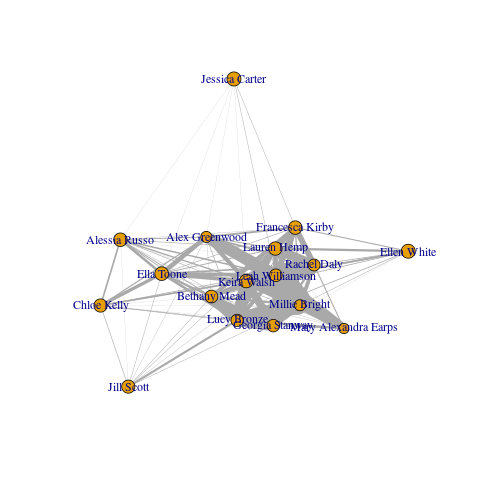
\includegraphics[width=\textwidth]{./img/plot_england_simpl.png}
   \caption{Red de pases total de Inglaterra simplificado en la EURO 2022}
   \label{img:red:simpl:eng}
\end{figure}

En \ref{img:ent:eng} estudiamos cómo es consistente con lo ya comentado, y hay poca variabilidad dentro de la 
entropía, conteniendo únicamente extremos mínimos correspondientes a la portera y máximos correspondientes a las defensas. 
Nos reafirma en que la entropía refleja bien el comportamiento en el campo, la posición de las jugadoras y cuántos 
minutos jugaron.

\begin{figure}[h!tbp]
  \centering
   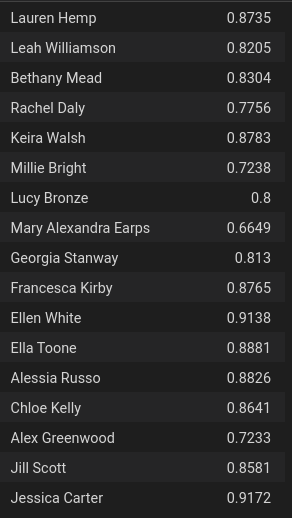
\includegraphics[width=\textwidth]{./img/entrop_engl.png}
   \caption{Entropía por jugadoras de Inglaterra en la EURO 2022}
   \label{img:ent:eng}
\end{figure}

En \ref{img:red:eng} vemos las redes de peso sin simplicar las aristas, lo que nos permite apreciar lo densa que es, pero a su 
vez están bien repartidas, y no apelotonadas como en Noruega \ref{img:red:norw}.

\begin{figure}[h!tbp]
  \centering
   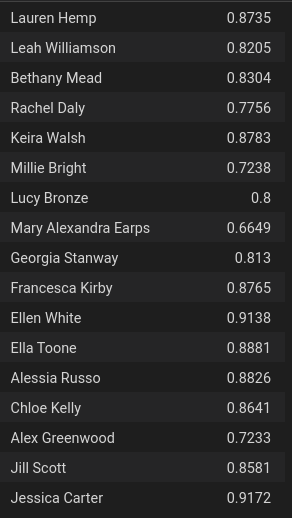
\includegraphics[width=\textwidth]{./img/entrop_engl.png}
   \caption{Entropía por jugadoras de Inglaterra en la EURO 2022}
   \label{img:red:eng}
\end{figure}

En \ref{img:red:simpl:nor} y \ref{img:red:nor} vemos que no es tanto una estructura casi romboidal, sino circular; 
están más juntas y sin una forma reticular clara.

\begin{figure}[h!tbp]
  \centering
   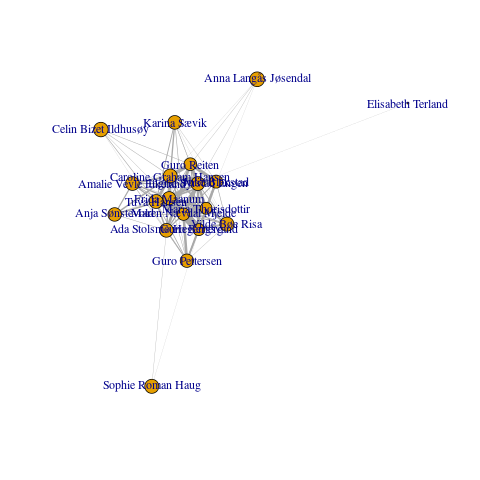
\includegraphics[width=\textwidth]{./img/plot_norw_simpl.png}
   \caption{Red de pases total simplificado de Noruega en la EURO 2022}
   \label{img:red:simpl:nor}
\end{figure}

\begin{figure}[h!tbp]
    \centering
     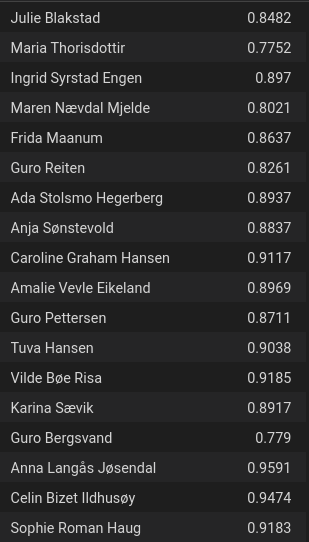
\includegraphics[width=\textwidth]{./img/entrop_norw.png}
     \caption{Entropía por jugadoras de Noruega en la EURO 2022}
     \label{img:red:nor}
\end{figure}

\begin{figure}[h!tbp]
    \centering
     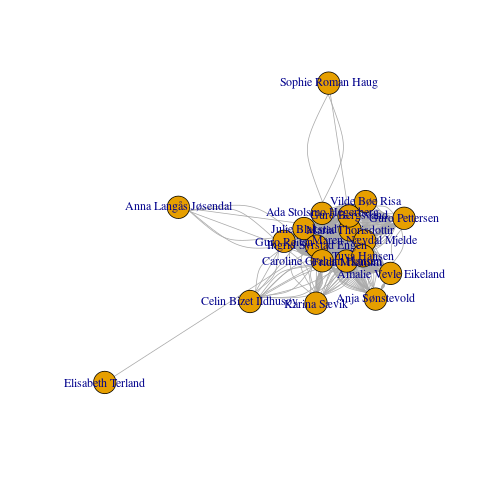
\includegraphics[width=\textwidth]{./img/plot_norw.png}
     \caption{Red de pases total de Noruega en la EURO 2022}
     \label{img:ent:norw}
\end{figure}

En \ref{img:fineng} y \ref{img:finnorw} vemos cómo Noruega se mantuvo con una entropía bastante alta en general
(lo que podemos ver reflejado en\ref{img:ent:norw}), 
mientras que la de Inglaterra es una curva decreciente, por lo que tienen orden y desorden, y consiguen un buen 
equilibrio.

\begin{figure}[h!tbp]
    \centering
     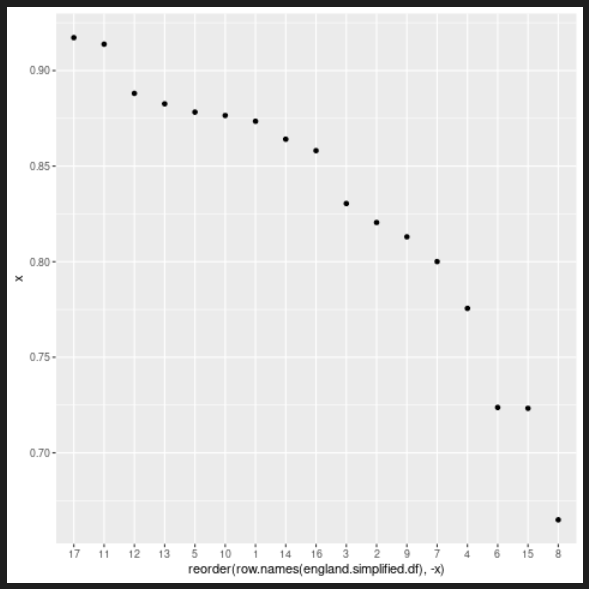
\includegraphics[width=\textwidth]{./img/englandentropy.png}
     \caption{Entropía de Inglaterra}
     \label{img:fineng}
\end{figure}

\begin{figure}[h!tbp]
    \centering
     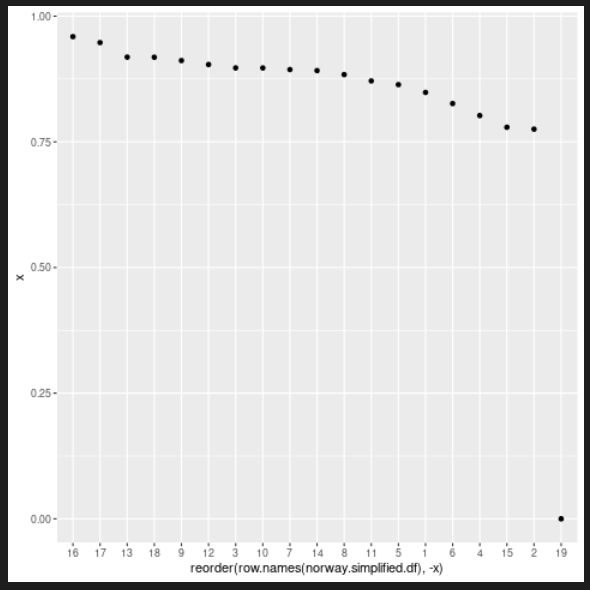
\includegraphics[width=\textwidth]{./img/norwayentrop.png}
     \caption{Entropía de Noruega}
     \label{img:finnorw}
\end{figure}

\section{Costes}
En cuanto a coste de amortización anuales, he usado mi portátil Asus Vivobook 14, comprado hace casi tres 
años por 799€, lo que se corresponde a 150€. El coste de desarrollo, teniendo en cuenta que 
hemos empleado 571 horas, entre 40 que son las horas que se echan por semana en un trabajo a 
tiempo completo, nos quedamos con 14 semanas, esto es, unos tres meses y medio. Si consultamos 
\href{https://www.linkedin.com/feed/}{LinkedIn}, las ofertas de trabajo para desarrolladores 
\textit{junior} están en torno a los 21.000€ al año, lo que viene a ser 1750€ por mes, añadiendo los 14€ 
que costaron el ventilador de Alehop mencionado en los agradecimientos. Esto se
muestra en la tabla \ref{tab:costes1}

\begin{table}
\begin{tabular}[h!tbp]{lccr}
  Concepto & Coste unitario & Unidades & Total \\
  Amortización portátil & 150€ & 1 & 150€ \\
  Ventilador            & 12€  & 1 & 14€ \\
  Costes laborales      & 1750€& 3.5 & 6125€ \\
  \hline \\
  \multicolumn{3}{l}{Total} & 6289€ \\
\end{tabular}
\caption{Costes el proyecto en el escenario ``ingeniera junior''} \label{tab:costes1}
\end{table}

Sin embargo, el trabajo realizado aquí corresponde más bien al de un analista
junior de datos deportivos. Según \href{https://www.payscale.com/}{Payscale}, el sueldo medio está en torno 
a los24000€. En este escenario los costes serían los indicados en la tabla \ref{tab:costes2}.

\begin{table}
\begin{tabular}[h!tbp]{lccr}
  Concepto & Coste unitario & Unidades & Total \\
  Amortización portátil & 150€ & 1 & 150€ \\
  Ventilador            & 12€  & 1 & 14€ \\
  Costes laborales      & 2000€& 3.5 & 7000€ \\
  \hline \\
  \multicolumn{3}{l}{Total} & 7164€ \\
\end{tabular}
\caption{Costes el proyecto en el escenario ``analista de datos junior''} \label{tab:costes2}
\end{table}

El coste de explotación, despliegue y producción se corresponderán a servicios de 
desarrollo a medida, adaptación, implantación, cursos, entre otros, pero este
tipo de trabajos se suelen hacer en nómina o bien vendiendo los informes; el
coste del informe trataría de ponerse de acorde con las horas empleadas y la
amortización del equipo durante el tiempo necesario. Una vez llevado a cabo todo
el análisis inicial y la exploración de los métodos, la elaboración de un nuevo
informe de este tipo se estima que duraría unos 15 días.

La biblioteca tendremos que 
mirarla cada cierto tiempo, actualizar dependencias, responder a los issues, para lo que echaremos 
40 horas al mes, que serán costes de producción que tendremos que factorizar en el coste del producto.


	% Presupuesto

	% Conclusiones
	\chapter{Conclusiones y trabajos futuros}



	% Trabajos futuros


	
	\newpage
	\bibliography{bibliografia}
	\bibliographystyle{plain}
	
\end{document}

